\chapter{Etude technique}

\section*{Inroduction}

\vspace{1cm \large Dans cette section, nous présentons en premier lieu l’architecture microservices et son utilité dans le monde informatique moderne. Puis, nous indiquons les technologies que nous utilisons pour réaliser notre travail ainsi que l’environnement de développement.}

\section{Architecture micro-services}

\vspace{1cm\large Micro-services est un style architectural qui représente un moyen de
concevoir les applications comme ensemble de services indépendamment
déployables. Ces services doivent de préférence être organisés autours des
compétences métier, de déploiement automatique, d'extrémités intelligentes et
de contrôle décentralisé des technologies et des données.}

\begin{figure}[H]
    \centering
    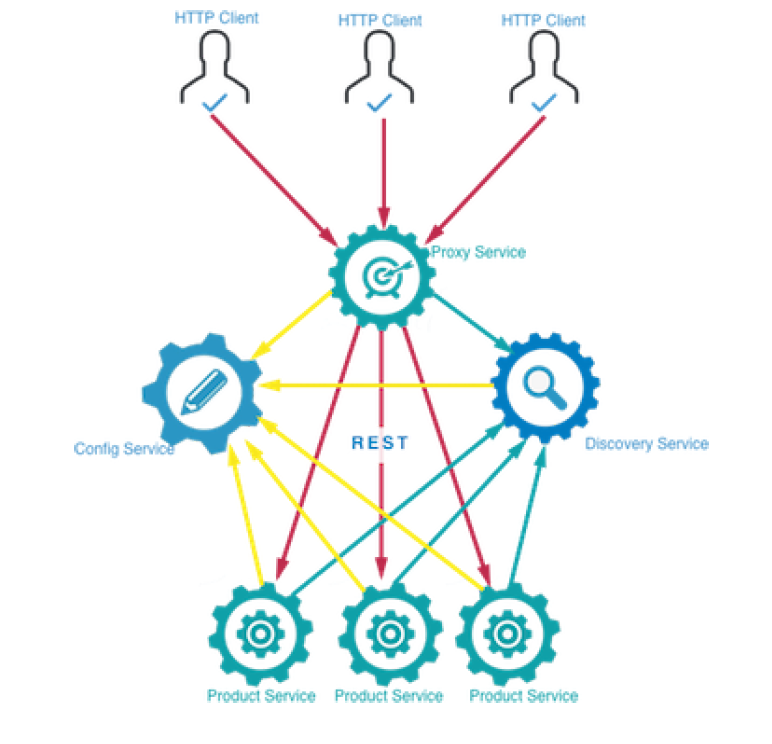
\includegraphics[width=0.7\columnwidth]{images/les12.PNG}
    \caption{Achitecture Microservice}
    \label{fig:Global}  
    \end{figure}
    \itemindent\textbf {\underline{Architecture}}
Cette architecture aborde le problème de la complexité
en décomposant l'application en un ensemble de services gérables qui sont beaucoup plus rapides
à développer et beaucoup plus faciles à comprendre et à maintenir. Cette architecture permet le développement de chaque service indépendamment l’un des autres par plusieurs équipes. De plus, elle réduit la barrière de l’adoption de nouvelles technologies puisque les développeurs sont libres de
choisir les technologies et ne sont pas limités aux choix faits au début du projet.
L’architecture microservices permet à chаque microservice d’être déployé indépendаmment. En conséquence, il rend possible le déploiement continu pour des applications complexes.

 \section{Technologies utilisées}
 \subsection{Les langages et Frameworks}
 Nous exposons, dans cette partie, les framework et les solutions technologiques nécessaires à la réalisation de notre projet et ce afin de satisfaire nos besoins fonctionnels et non fonctionnels.
 
 \begin{table}[H]
    \captionsetup{justification=centering}
    \caption{  \label{tab:UC-ATH} Tableau résumant les technologies utilisées dans notre projet.}
    \centering
    \begin{tabular} {|m{10em}|m{25em}|}
    \hline
    \rowcolor[HTML]{8c9eff} 
    \textbf{ } & \textbf{Technologie} \\
    \hline
    \rowcolor[HTML]{e8eaf6}
    \textbf{Backend} & JAVA8, SPRING BOOT, SPRING CLOUD, MAVEN, Bamboo \\
    \hline
    \rowcolor[HTML]{f3e5f5}
    \textbf{Frontend} & Angular, HTML5, CSS3 et Typescript. \\
    \hline
    \rowcolor[HTML]{e8eaf6}
    \textbf{BDD} & NoSQL, Cassandra \\ 
    \hline
    \rowcolor[HTML]{f3e5f5}
    \textbf{Méthodologies} & Agile SCRUM. \\ 
    \hline
    \rowcolor[HTML]{e8eaf6}
    \textbf{DEVOPS} & JIRA, GitLab, SonarLint.\\
    \hline
    \end{tabular}
    \end{table}
    
    \subsubsection{JAVA8}
    Java 8 est la dernière version stable de Java qui offre de nouvelles fonctionnalités, desperformances accrues et des corrections de bug pour améliorer l’efficacité de développementet d’exécution des programmes Java.Les nouvelles fonctionnalités de Java 8 :\\
    \noindent \textbf{-Expression lambda et méthodes d’extension virtuelle :} programmation fonctionnellepour un code plus simple et plus compact.\\
    \noindent \textbf{-API de date/heure :} facilite la gestion de la date et de l’heure de façon plus naturelle,simple et compréhensible.\\
     \noindent \textbf{-fMoteur JavaScript Nashorn :}exécution du code Javascript dans Java.\\
   \noindent \textbf{-Encodage Base64 :}pour la sécurité.\\
     \subsubsection{SPRING BOOT}
    
    Spring est le framework de développement d’applications le plus populaire. Il est né de l’idée de fournir une solution plus simple et plus légère que celle proposée par Java 2 EE. permet de son côté de construire des applications Spring rapidement aussi rapidement que possible, en minimisant au maximum le temps de configuration, d'habitude
pénible.

                  
                  \subsubsection{ANGULAR}
                  Angular est une plateforme de développement qui permet de créer des applications web dynamiques et immersives.  Dans ce cours, vous apprendrez rapidement à créer les composantes de base d'une application Angular, avant d'enrichir vos applications en approfondissant vos connaissances de ce framework.  Vous apprendrez également à faire communiquer votre application avec un backend afin de créer une application web complète.
                  
                   \subsubsection{Cassandra (base de données)}
                   Apache Cassandra est un système de gestion de base de données (SGBD) de type NoSQL conçu pour gérer des quantités massives de données sur un grand nombre de serveurs, assurant une haute disponibilité en éliminant les points individuels de défaillance. Il permet une répartition robuste sur plusieurs centres de données4, avec une réplication asynchrone sans master et une faible latence pour les opérations de tous les clients.
                   \subsubsection{Bamboo}
                   Bamboo est un outil Open-Source d’Intégration Continue, le principe est de vérifier, idéalement à chaque modification de code source, que le
résultat de ces modifications de produit pas de régression sur l’application, la mise en commun entre développeurs se fait à chaque
modification/commit, en continu ; ce qui permet d’augmenter les chances que chaque portion de l’application fonctionne avec ses autres
composantes.
                  
                  
































    \subsection{Environnement logiciel}
    
    \subsubsection{Spring Tool Suite (STS 4): Backend}
    
   STS est un environnement de développement basé sur Eclipse qui est personnalisé pour le développement d'applications Spring.

Il fournit un environnement prêt à l'emploi pour implémenter, déboguer, exécuter et déployer vos applications. Il inclut également une intégration pour Pivotal tc Server, Pivotal Cloud Foundry, Git, Maven et AspectJ. STS s’ajoute aux dernières versions d’Eclipse.
    
    \subsubsection{WebStorm 11: Frontend}
    WebStorm est un IDE pour les langages Web (HTML, CSS et JavaScript), développé par l'entreprise JetBrains et basé sur la plateforme IntelliJ IDEA
    

    
    \subsubsection{JIRA}
    
    C’est un logiciel pour la gestion de projets pour les équipes agiles. Il permet de gérer le backlog produit, les sprints ainsi que les tickets. De plus il permet d’établir des rapports pour se bénéficier des informations en temps réel par rapport à l’avancement et du temps consommé par tâche .
    
    \subsubsection{SourceTree}
    SourceTree simplifie la façon dont vous interagissez avec vos référentiels Git afin que vous puissiez vous concentrer sur le codage. Visualisez et gérez vos référentiels via une interface simple.
    
    \subsubsection{DevCentre}
    DataStax DevCenter est un IDE visuel gratuit de schémas et de requêtes destiné aux développeurs, administrateurs et autres personnes souhaitant créer et exécuter des instructions CQL (Cassandra Query Language) sur Apache Cassandra et DataStax Enterprise. Les utilisateurs peuvent rapidement ajouter et créer de nouvelles connexions, importer des requêtes précédemment enregistrées et naviguer dans des instances de base de données. 
    
     \subsubsection{Postman}
Postman est un logiciel qui se focalise sur les tests des API. Il est devenu très populaire pour tester les Microservices, notamment grâce à sa simplicité et ses fonctionnalités très spécialisées.
\subsubsection{StarUML}
C’est un logiciel de modélisation qui prend en charge la modélisation agile. Il offre la
possibilité de modéliser plusieurs types de diagrammes tel que le diagramme de cas d’utilisation,
diagrammes de séquences et diagrammes de classes


\section{Architecture de l'environnement du travail}
    \subsection{Architecture physique}
    Pour l'architecture physique de notre projet, nous avons décidé de mettre en place une architecture microservice, c'est l'architecture qui convient le mieux avec nos besoins. 
Nous allons donc créer les microservices suivants:
\begin{itemize}[font=\normalsize]
                  \ding{226}\textbf{ Product Service :}Service principal, qui offre une API REST pour lister une
liste de produits
                  \end{itemize} .
                  
                  \begin{itemize}[font=\normalsize]
                  \ding{226}\textbf{ Config Service :}Service de configuration, dont le rôle est de centraliser les
fichiers de configuration des différents microservices dans un endroit
unique.
                  \end{itemize} .
                  \begin{figure}[H]
        \centering
        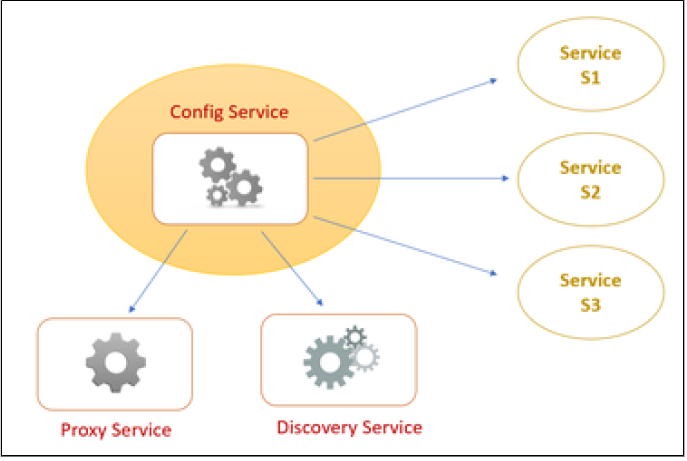
\includegraphics[width=1\columnwidth,height=0.5
\columnwidth]{images/config.PNG}
        \caption{Microservice Config-Service}
        \end{figure}
        \newpage
        
                  \begin{itemize}[font=\normalsize]
                  \ding{226}\textbf{ Proxy Service :}Passerelle se chargeant du routage d'une requête vers l'une
des instances d'un service, de manière à gérer automatiquement la
distribution de charge.
                  \end{itemize} 
                   \begin{figure}[H]
        \centering
        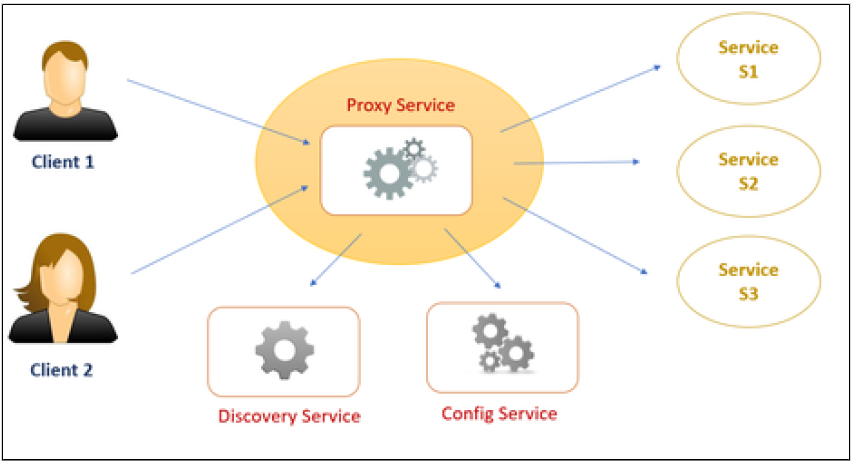
\includegraphics[width=1\columnwidth,height=0.4
\columnwidth]{images/proxy.PNG}
        \caption{Microservice Proxy-Service}
        \end{figure}.
                  \begin{itemize}[font=\normalsize]
                  \ding{226}\textbf{ Discovery Service :}Service permettant l'enregistrement des instances de
services en vue d'être découvertes par d'autres services.
                  \end{itemize} .
                  \begin{figure}[H]
        \centering
        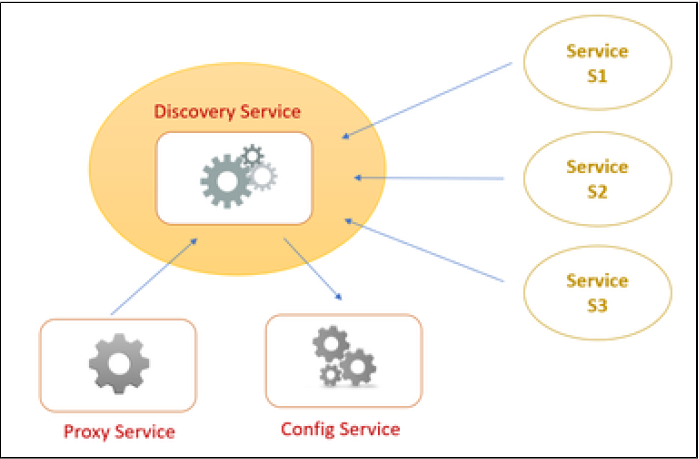
\includegraphics[width=1\columnwidth,height=0.4
\columnwidth]{images/discovery.PNG}
        \caption{Microservice Discovery-Service}
        \end{figure}
        \subsection{Structure d'un microservice}
                   \begin{figure}[H]
        \centering
        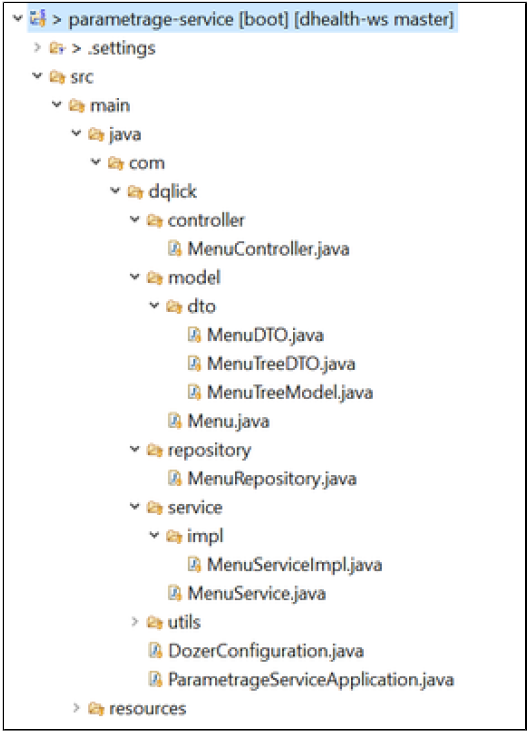
\includegraphics[width=0.8\columnwidth,height=1
\columnwidth]{images/structure.png}
        \caption{Structure d'un microservice}
        \end{figure}
    
  

\section*{Conclusion}
Dans ce chapitre, nous avons fait une étude sur les technologies que nous allons utiliser pour la réalisation de notre projet et nous avons dressé l'architecture physique de notre projet.